% !TEX root = ../report.tex

\section{Design}\label{design}
\thispagestyle{plain}

\subsection{Mechanical design decisions}\label{design/mechanical}

The mechanical design of each agent is central to its functionality, with sensors being heavily reliant on the accuracy of the mechanical
construction. As multiple robots are being created, the mechanical similarity is
also important to ensure the sensors and software function consistently across each robot. The placement of sensors will be critical to this and
so the first robot will be completed and tested before further agents are constructed.
Printed Circuit Boards (PCBs) are likely to be used for this purpose in the
final iteration of the design---with strip board being used for prototyping---as this will provide additional robustness and guaranteed
repeatability between robots.

\subsubsection{Chassis and motors}\label{design/mechanical/chassis}

The main design decision to be made involving the chassis was whether to
use a pre-built ``hobbyist'' chassis or create a bespoke design which could
be easily replicated for each agent. The initial design plan had been to
use pre-built chassis with the primary concern regarding this was that
motors were often included in these pre-built packages and these motors
could be insufficient for wheel odometry purposes.

Following a consultant meeting with Dr Mark Post (see Section~\ref{plan/structure}),
it was suggested that a bespoke chassis may better fit
the requirements of the task. This sentiment was echoed by Dr Harle in a
class meeting when it was suggested that mechanical assistance was readily
available from the mechanical workshop in the EEE department. In order to
do this, a CAD (Computer Aided Design) model would have to be created and
taken to the mechanical workshop for a model to be either laser cut or 3D
printed.

Chassis selection became integral to the flow of the project as a
bespoke design would have to be created last in the design process
following the detailed design of other aspects such as the sensor layout
and PCB design, whereas a pre-built chassis could be used to prototype
design solutions prior to a final design decision.

These options were considered against each other and it was decided
that a pre-built chassis would be used due to a number of factors, namely:
the lack of in-depth knowledge of CAD amongst the team; the possible cost
of a bespoke chassis compared to pre-built; and the lack of control
surrounding the creation of the chassis. Having weighed the pros and cons
of each approach it was concluded that the cons of designing a bespoke
chassis outweighed the pros and so a pre-built chassis would be used. This
will be ordered in the coming weeks as per the Gantt chart (Figure~\ref{figure:gantt}).

Having investigated multiple possible options, two-wheeled robots were
found to be the simplest and most mechanically simple to work with while
providing the required precision of movement. Many of these chassis are
accompanied by motors which would be sufficient for the purposes required.
One particluar example chassis~\cite{pololuchassis} is  accompanied by two
motors with sufficient gearing (120:1) to allow for the required precision
when driving the robot. This chassis also has a number of additional
accompanying parts which will be useful in maintaining both mechanical
stability and a high level of repeatability.


\subsubsection{Drive system}\label{design/mechanical/drive}

The drive system for the robots will be a differential drive system (DDR).
This drives each wheel independently using independent actuators and the
wheels are not connected by a single axle~\cite[p.~146]{braunl_embedded_2013}.
When using a two wheeled robot, DDR allows the
robot to rotate on the spot around its central axis when the wheels are
driven in opposite directions. This provides a high level of mobility which
will aid in the sensing and mapping capabilities of the robot. Each wheel
will require a individual motor and an encoder for wheel odometry data.

The drive system will be controlled either by the central computer on
the Raspberry Pi or by a microcontroller uniquely assigned to managing the
drive system. In either case the wheel odometry data will be gathered and
sent for fusion with data from other sensors on the Raspberry Pi for the
purpose of localisation. The benefits of using a microcontroller for the
drive system would predominantly be the higher level of precision with
which tasks could be timed and carried out. This would also allow the
odometry data to be collected quickly and regularly with little
interference from other tasks, ensuring the data was correct. The decision
on this has not yet been made and this will be based predominantly on the
load of the algorithms on the Raspberry Pi which is currently difficult to
determine. A cheap and effective microcontroller such as the MSP430
Launchpad could be ordered and integrated at fairly short notice following consultation with Dr James Irvine (see Section~\ref{plan/structure}).

A pre-built motor drive board is likely to be used from the same supplier as the
pre-built chassis. As an
accompanying component the circuit is guaranteed to fit neatly onto the
chassis~\cite{pololudriver}. This circuit also includes a power distribution board
which will be useful in reducing the mechanical complexity of the robot.
Using these pre-built solutions will improve the repeatability of the
robot as the number of parts which have to be created and fitted will be
reduced.

\subsubsection{Mechanical conclusions}\label{design/mechanical/conclusion}
A number of pre-built solutions have been chosen for the mechanics of the
robot as the consistency between robots is vital to their coordination and
although bespoke solutions may have provided a small increase in
consistency, these would have required a disproportionate amount of design
and implementation time in an aspect of the project which is not a novel
concept. A sharp learning curve would also be involved in creating
bespoke mechanics, and while alone this is not as bad thing it would be
accompanied by the sharp learning curves of SLAM and computer vision. It
was therefore decided that pre-built parts should be used and time of the
project diverted towards those areas instead.

The main objectives for this mechanical design are therefore as follows:
\begin{itemize}
    \item{Construct an easily replicable robot}
    \item{Use predominantly pre-built components with PCBs to maintain consistency}
    \item{Order pre-built components as per Gantt chart Figure~\ref{figure:gantt}}
\end{itemize}

\subsection{Sensor selection}\label{design/sensors}

\subsubsection{Range sensing}

Localisation requires a sensor or set of sensors capable of measuring the
distance to objects in the robot's environment. The primary range sensors considered for this
project are all active sensors, meaning that they measure the echo from a transmitted
signal. Range-finding sensors of this sort include infrared range-finders, ultrasonic
transceivers, and lidar.

Of these, lidar gives the most accurate readings, and has the advantage of
covering \ang{360}. However, the most affordable lidar systems exceed the budget
of the project and are too large to be placed on the chassis. For these reasons,
lidar was immediately discounted as a possibility for our application.

Infrared range-finders form an inexpensive alternative to lidar. Here, a narrow
beam of infrared light is emitted, and the distance is determined by trigonometric
calculations based on the angle of reflection. The main disadvantages of these
sensors is a significant decrease in reliability, due partly to the possibility that
the narrow light beam may not detect objects that take up a small proportion
of the field of view, and partly to the risk of interference by other light
sources~\cite{herbert00}.

Ultrasonic transceivers are another inexpensive option. This sensor
consists of a transceiver which transmits and receives ultrasound pulses of a
specific frequency. By measuring the time delay between transmitting and
receiving, the distance to an object which is reflecting the signal can be
calculated. At a low price range, ultrasonic sensors result in less accurate
readings than infrared sensors; however, the wider effectual angle of these sensors
combined with the advantage that they are not affected by ambient light or the
reflectance or gloss of materials make them significantly more reliable in many
circumstances.

Ultrasonic sensors have a minimum range, below which they are prone to incorrect
measurements caused by registering subsequent echoes. This ``deadband'' distance is
typically in the range of less than \SI{3}{\cm}. In order to avoid the
possibility of objects appearing within this range, the sensors need to be set
back from the edge of the robot, so that objects directly adjacent to the robot
fall within the material window of the sensor.

The maximum range of ultrasonic sensors varies between sensor models, and further
depends on the size and material of the object being detected. A practical sensor
range of around \SI{1}{\m} is typical for low-budget sensors. As the robots will be
operating in a controlled environment for the purposes of this project, the maximum
distance of an object within the environment can be controlled.

Ultrasonic sensors can only detect objects that fall within the conical beam emitted
by the transmitter. The measuring angle of this beam is typically around \ang{15}.
In order to identify objects in a wider field of view, multiple sensors need to be
arranged around the robot. Our intention is to use between three and five sensors
on each robot, spaced at between \ang{20} and \ang{30} to create a field of view
of around \ang{90} to \ang{120}, facing towards the front of the robot as shown in Figure \ref{UltraSoundSensorDiagram}.

\begin{figure}[!ht]
	\centering
	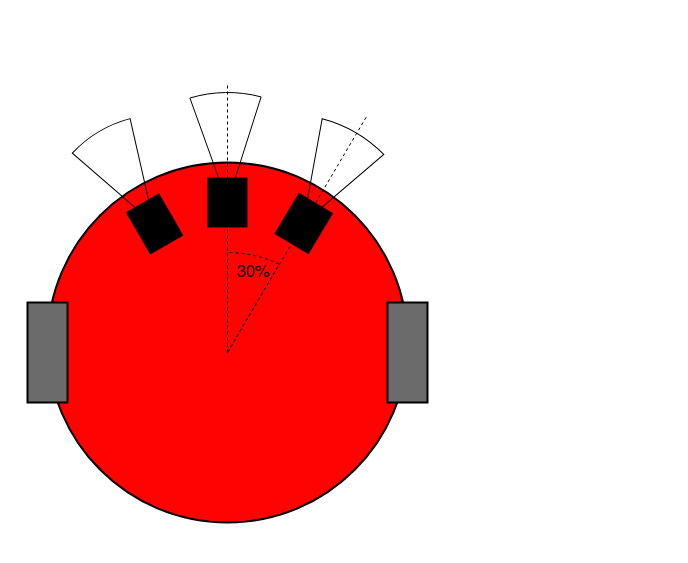
\includegraphics[width=0.5\textwidth]{UltraSoundSensorDiagram}
	\caption{Ultrasound Sensor Layout}\label{UltraSoundSensorDiagram}

\end{figure}

One drawback of using active range-finders is that there is the possibility that
sensors will interfere with each other. This problem is normally solved by
synchronising the sensors so that they fire alternately, ignoring any signals
received outwith a specified time period. Synchronising ultrasonic sensors on a
single robot is a trivial task; however, synchronising between robots will require
some coordination which will be discussed further in Section~\ref{design/software/comms}.


\subsubsection{Inertial Measurement Unit}
A 6 degree of freedom (dof) IMU measures both its acceleration in 3 axes and its angular velocity in about these axes. This allows the robot to keep track of its position and orientation relative to where it started over time.

The IMU currently being used is the MPU-6050. At its smallest range of accuracy ($\pm250^\circ$/s and $\pm2g$\cite{MPU6050Datasheet}, which will be adequate for our application) it was the most accurate sensor available at a similar budget in terms of non-linearity, cross-axis sensitivity and noise. Offset tolerance was not a major consideration as calibration can compensate for this, as long as it is not so significant that it can reduce the range. In terms of power consumption, while it was not the most efficient, it was reasonable, and power is not a major constraint of the project. Additionally, it performs some on board computation with the results, easing the load in interpreting the raw data for the control system.

A major problem with using the IMU is that as it has to integrate the rotational velocity and double integrate the acceleration to track the position, small errors or offsets can accumulate over time and cause a large ``drift'' in the estimated position.


\subsubsection{Encoder hardware}\label{design/sensors/encoder}

An encoder is a feedback device which can be connected to motors to provide
sensing data, such as the wheel speed and position, which can aid in localisation~\cite[p.~60]{braunl_embedded_2013}.
There are two main types of encoder, namely: linear, which senses motion along
a fixed path, and rotary, which senses rotational motion~\cite[p.~60]{braunl_embedded_2013}.
As the robot will use wheels to move, a rotational encoder for each wheel will be used.
There are a further two sub-types of rotational encoder: incremental rotary encoders and absolute rotary encoders. The incremental encoders considered use light and a glass disk to generate a series of
pulses. The position of the incremental encoder is determined using the pulses produced.
They are not as accurate as the other form of rotary encoder: absolute encoders.
Absolute encoders also use light to detect movement, however these use a
stationary mask giving each position its own unique set of bits.

A number of factors influence the selection of encoders including the output
type, the desired resolution, and the size of the encoder and casing. Since a pre-built
chassis will be used, the size of the encoder is the most high priority requirement as
it must fit onto the body of the robot. The desired resolution is also important due to
the lack of accurate sensors for mapping (see Section~\ref{design/sensors}), wheel odometry will be
of greater importance for localisation, hence it is important that this is accurate.
With a few exceptions, absolute encoders are significantly more expensive than
incremental encoders and so it is likely that incremental encoders will be used for
this project.

If using the expected pre-built chassis~\cite{pololuchassis},
this also comes with accompanying encoders~\cite{pololuencoder}.
These will be used as they are made specifically for the pre-built chassis and operate in the
correct revolutions per minute (rpm) to match the motors provided with the chassis and a high number of counts per revolution providing high levels of accuracy.

\subsection{Software design}\label{design/software}

\subsubsection{Software engineering practices and structure}
In considering frameworks and tools to apply to the project, there are
several key decisions to be made, crucially in software architecture style
and language choice.

In the high level structure of the software, several architectures might be
employed. The highly modular nature of the system, with many interacting
components each having very specific functions, lends itself especially well
to an Object Oriented or Implicit Invocation architecture. The object
oriented paradigm is well known, abstracting the system into smaller
functional groups called objects which invoke each other's methods. Perhaps
less well known, the event driven implicit invocation paradigm is very
similar to object oriented design, but with the crucial difference that
objects do not interact by directly calling each other, but rather by
observing each other for events that require a response. This change is well
suited to this project, as many of the modules will be constantly outputting
data (such as the sensors) or else performing analysis of new data (such as
SLAM) and all performing in parallel.

Another important consideration is which programming languages to utilise for
the project. The main possibilities are Python, which is well supported by
the Raspberry Pi and easy to use, allowing for rapid prototyping and
development, and C/C++, which is more difficult to develop in but leads to
more efficient programs.

A solution to both of these dilemmas is presented by using the Robot
Operating System (ROS) framework. ROS is an open-source programming framework
for complex modular robotic networks. It is not an operating system as such,
despite the name, but rather a collection of libraries and tools to make it
easier to develop modules within a robot and allow them to communicate.

The framework treats the robot as a network of nodes (individual programs
with one or few purposes). Nodes communicate via a modified version of the
Observer design pattern known as the Publish/Subscribe model. Data is
attached to a \emph{``Topic''}, which is published by a node. Any number of
nodes can subscribe to a topic, and when data is published on that topic an
interrupt function is triggered in the Subscriber node, allowing access to
the data.

ROS creates very loose coupling between nodes, which promotes good software
engineering practices, and will allow the system to be easily modified and
expanded. This also makes testing far easier, as modules can be unit tested
on their own and integrated together after the fact.

All this is to say that by utilising the framework and implementing modules
as ROS nodes, the high level architecture of the system becomes very much
akin to implicit invocation. Moreover, ROS supports nodes within the same
system being programmed in several languages, including Python, C++ and Java,
meaning that this decision can be made on a module by module basis.

With this in mind, the high level architecture of the system is shown in
figure \ref{figure:architecture}, with each block in the diagram representing
a ROS node, and each arrow corresponding to communication of a topic between
those nodes.

\begin{figure}[ht]
    \centering
    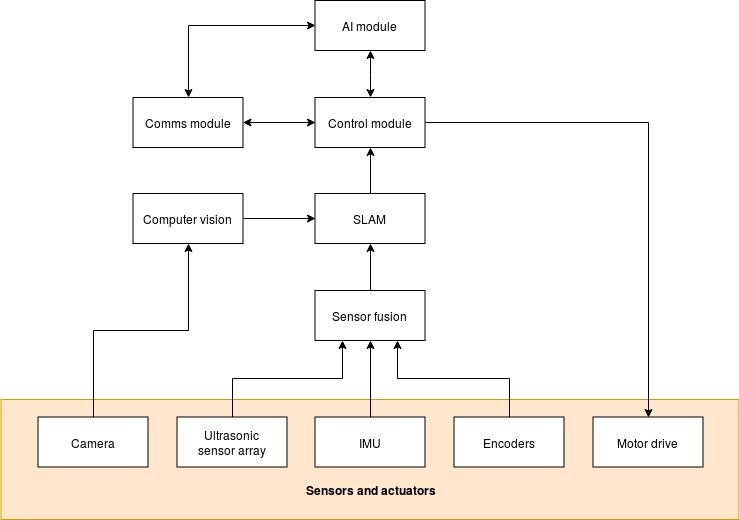
\includegraphics[width=0.8\linewidth]{software_diagram.png}
    \caption{High-level module diagram of software components}
    \label{figure:architecture}
\end{figure}


\subsubsection{SLAM and sensor fusion}
Implementing SLAM is one of the key challenges of the project. The two main
options are either to create an implementation from scratch or to use an
existing library or framework to aid in providing this functionality for the
robots. An example of such a library is PythonRobotics, which contains a
collection of robotics algorithms, especially with the focus for use in
autonomous navigation. There are also libraries for use with ROS that could be used to implement the SLAM such as ``gmapping''.

FastSLAM is a commonly used implementation, a factored solution first proposed in~\cite{montemerlo2002fastslam}. This involves recursively estimating the full
posterior distribution over the robot's pose and landmark locations, but scales
logarithmically over the number of landmarks in the map. This, therefore, is
very scalable and thus used for areas with a greater number of landmarks---it
was tested up to 50,000 landmarks initially. An improvement to the algorithm was
released as FastSLAM 2.0~\cite{montemerlo2007fastslam}. An issue found in the
original FastSLAM algorithm was that the performance degraded if the sensors were
too accurate and the motion uncertainty was too great relative to the
observations. FastSLAM 2.0 utilises the current observation when creating the
proposal distribution to create better matches and improve its accuracy. As a
result, the original algorithm is worse in nearly all aspects with the main disadvantage being that FastSLAM 2.0 is more difficult to implement.

The alternative implementation approach considered was to write an implementation
from scratch without the use of any frameworks. This would have the advantage that the solution would be fully customised to the needs of the project. Alternatively, however,
SLAM in itself is a difficult concept and so it may not be feasible in the time to
implement it successfully.

The implementation of SLAM will most likely involve using FastSLAM, or an equivalent
implementation algorithm. This is because, even when using such a library, this is already a very challenging
problem. Implementing SLAM from scratch would likely prove very difficult to manage in
the time constraints of the project, especially when it is only part of the full
solution. Both the input to and the output from the framework will need altered and
analysed before the robot can interpret where they are and create a map which will likely be difficult.

\subsubsection{Computer vision}

Solutions both using computer vision and relying on other sensor types were discussed.
While it can be computationally intensive, especially for the microcomputers that we
intend to use, computer vision can provide the system with a wealth of useful information,
is more flexible than most other practical sensors, and provides unique solutions to
several problems encountered in this project.

Firstly, a monocular, feature-based object identification system could be used to
implement loop closure when mapping the environment. This can drastically reduce error,
especially over larger areas, where drift is most prolific.

This could also be used for the identification of other robots. This then allows the
system to not map the robots in the environment and identify what other robots are
doing and coordinate itself without direct communication.

If the CV system was bi-ocular, it could also be used for measuring distance, and
could perhaps replace or improve the distance sensing system.

It was decided that the monocular solution was to be implemented as it would allow
loop closure and robot identification, which would otherwise be very difficult. The
two-camera solution would be far more computationally expensive than using
ultrasound distance sensors.

There are several distinct types of feature detection that can be used for SLAM, each
with their own key point detection and feature description algorithms. In a quantitative
comparison of several different algorithms (SIFT, SURF, KAZE, AKAZE, ORB, and BRISK),
it was found that ORB is the most efficient, with BRISK slightly slower, which also
proves to be the most accurate~\cite{FeatureBasedComparison} (with the exception of
SIFT, however this is not appropriate given the licensing requirements). Therefore either ORB or BRISK will be used going forward. It is currently expected
that ORB will be used, as BRISK's performance benefits are only significant when
there are large changes in scale or rotation~\cite{FeatureBasedComparison}, which is not expected given our application.

It should be noted that while an ideal solution would implement a system as described,
due to time constraints and the focus of the project on the co-operative
performance, a simpler method of simulating this behaviour may be used, such as
identifying robots by colour.

Research was also conducted into the hardware required for the computer vision. As the processing will be done on a Raspberry Pi (RPi) zero, it was decided to use the standard RPi camera. This allows the use of the RPi's dedicated Camera Serial Interface (CSI) port instead of the USB ports that would be required by most alternatives. This reduces the computation required by both the camera and, more importantly, the RPi.

\subsubsection{Communication}\label{design/software/comms}

The requirement that robots can only communicate when they have line-of-sight poses
severe restrictions on the types of communication that can be performed. While the
robots will be operating in a small enough area that it will always be possible for
them to communicate with all other robots, we will be artificially restricting their
ability to communicate in order to simulate an environment in which physical limitations
apply.

Communication may be performed using either Wi-Fi or Bluetooth. At present, the most
promising solution appears to be a wireless ad-hoc network (WANET), which allows the
robots to communicate directly with each other using Wi-Fi without the need to connect
to a router. This has the added advantage that all nodes on the network are equal.
For debugging and monitoring purposes, the robots may also be communicate with a
computer on the same network.

\subsubsection{AI and control modules}\label{design/software/ai}

A central control module will interact with the low-level systems and coordinate the
robots' sensors and actuators. High-level decisions about how to navigate the environment
will be made by a separate AI module, which will interact with the communications
system to coordinate the search of the map with other robots.

Basic algorithms for exploring a physical maze-like environment include depth-first
search, where the robot continually takes arbitrary paths until it reaches a dead end
or encounters a previously explored position again, and then doubles back to the last
fork in the maze and takes the next unexplored path, as shown in Figure~\ref{figure:maze/a}.
This algorithm will always terminate on a finite maze.

Given multiple robots, this algorithm can be extended to search a space more efficiently.
By travelling together until they encounter a fork and then splitting up, they can
potentially explore the environment significantly quicker (Figure~\ref{figure:maze/b}).

\begin{figure*}[t!]
    \centering
    \begin{subfigure}[t]{0.5\textwidth}
        \centering
        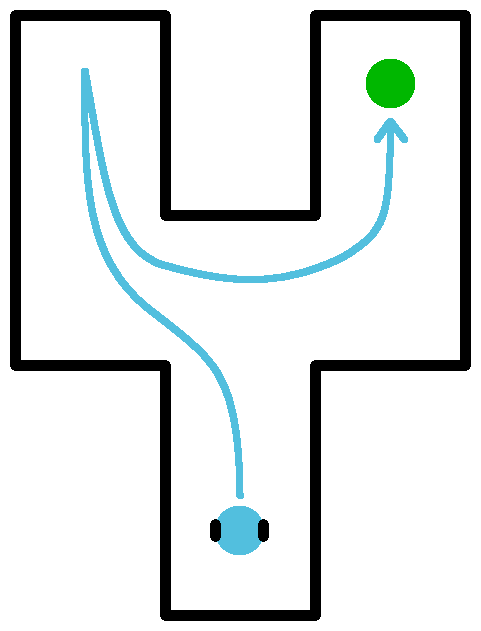
\includegraphics[width=0.6\linewidth]{maze_a.png}
        \caption{One robot solving the maze using depth-first search}\label{figure:maze/a}
    \end{subfigure}%
    ~
    \begin{subfigure}[t]{0.5\textwidth}
        \centering
        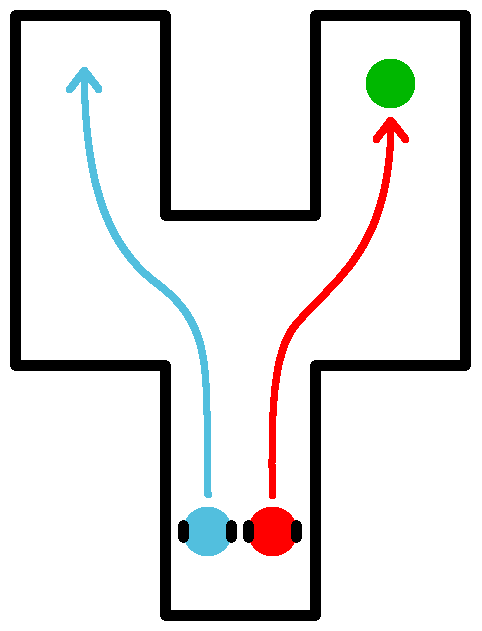
\includegraphics[width=0.6\linewidth]{maze_b.png}
        \caption{Two robots co-operatively solving the same maze}\label{figure:maze/b}
    \end{subfigure}
    \caption{Example of robots solving a simple maze}
\end{figure*}

To allow the system to be modified and extended, the control module should be implemented as a rich API, allowing the AI to be easily rewritten by abstracting the robot to a single external interface.

\subsection{Software conclusions}\label{design/software/conclusion}
Utilising ROS as the underlying framework, and programming in any language deemed reasonable for the specific module, several key modules must be implemented. A computer vision module must be created, and integrated with a module implementing SLAM for the robot. Moreover, a communication system will be implemented to allow the robots to interact with each other. Finally, a central control module must be devised, as well as an AI module which can interact with the system as an API.
